\documentclass[11pt]{article}
\usepackage{wasysym}
\usepackage{listings}
\usepackage{tikz}
\usepackage{url}
%\usepackage{algorithm2e}
\usetikzlibrary{arrows,automata,shapes}
\tikzstyle{block} = [rectangle, draw, fill=blue!20, 
    text width=2.5em, text centered, rounded corners, minimum height=2em]
\tikzstyle{bw} = [rectangle, draw, fill=blue!20, 
    text width=3.5em, text centered, rounded corners, minimum height=2em]

\newcommand{\handout}[5]{
  \noindent
  \begin{center}
  \framebox{
    \vbox{
      \hbox to 5.78in { {\bf ECE459: Programming for Performance } \hfill #2 }
      \vspace{4mm}
      \hbox to 5.78in { {\Large \hfill #5  \hfill} }
      \vspace{2mm}
      \hbox to 5.78in { {\em #3 \hfill #4} }
    }
  }
  \end{center}
  \vspace*{4mm}
}

\newcommand{\lecture}[4]{\handout{#1}{#2}{#3}{#4}{Lecture #1}}
\topmargin 0pt
\advance \topmargin by -\headheight
\advance \topmargin by -\headsep
\textheight 8.9in
\oddsidemargin 0pt
\evensidemargin \oddsidemargin
\marginparwidth 0.5in
\textwidth 6.5in

\parindent 0in
\parskip 1.5ex
%\renewcommand{\baselinestretch}{1.25}

\begin{document}

\lecture{2 --- January 7, 2015}{Winter 2015}{Patrick Lam}{version 1}

\section*{Modern Processors}

I asked you to watch the video by Cliff Click on modern
hardware:

\begin{center}
\url{http://www.infoq.com/presentations/click-crash-course-modern-hardware}
\end{center}

Cliff Click said that 5\% miss rates dominate performance. Let's look at why.
I looked up a characterization of the SPEC CPU2000 and CPU2006 
benchmarks\footnote{A. Kejariwal et al. ``Comparative architectural characterization of SPEC CPU2000 and CPU2006 benchmarks on the Intel Core 2 Duo processor'', SAMOS 2008.}.

Here are the reported cache miss rates\footnote{\permil~is ``permil'', or per-1000.} for SPEC CPU2006.

\begin{center}
\begin{tabular}{ll}
L1D & 40\permil \\
L2 & 4 \permil
\end{tabular}
\end{center}

Let's assume that the L1D cache miss penalty is 5 cycles and the L2 miss penalty is
300 cycles, as in the video. Then, for every instruction, you would expect a running
time of, on average:
\[ 1 + 0.04 \times 5 + 0.004 \times 300 = 2.4. \]
Misses are expensive!

\paragraph{Forcing branch mispredicts.} It takes a bit of trickery to force branch
mispredicts. {\tt gcc} extensions allow hinting, but usually {\tt gcc} or the processor
is smart enough to ignore bad hints. This\footnote{Source: \url{blog.man7.org/2012/10/how-much-do-builtinexpect-likely-and.html}.} worked last year, though:

{\tiny
\begin{verbatim}
        #include <stdlib.h>
        #include <stdio.h>

        static __attribute__ ((noinline)) int f(int a) { return a; }

        #define BSIZE 1000000
        int main(int argc, char* argv[]) 
        {
          int *p = calloc(BSIZE, sizeof(int));
          int j, k, m1 = 0, m2 = 0;
          for (j = 0; j < 1000; j++) {
            for (k = 0; k < BSIZE; k++) {
              if (__builtin_expect(p[k], EXPECT_RESULT)) {
                m1 = f(++m1);
              } else {
                m2 = f(++m2);
              }
            }
          }

          printf("%d, %d\n", m1, m2);
        }
\end{verbatim}
}
Running it yielded:
\begin{verbatim}
plam@plym:~/459$ gcc -O2 likely-simplified.c -DEXPECT_RESULT=0 -o likely-simplified
plam@plym:~/459$ time ./likely-simplified
0, 1000000000

real	0m2.521s
user	0m2.496s
sys	0m0.000s
plam@plym:~/459$ gcc -O2 likely-simplified.c -DEXPECT_RESULT=1 -o likely-simplified
plam@plym:~/459$ time ./likely-simplified
0, 1000000000

real	0m3.938s
user	0m3.868s
sys	0m0.000s
\end{verbatim}
{\tt gcc} seems to have gotten smart enough to reject bogus hints in the interim.

\section*{Limits to parallelization}
I mentioned briefly in Lecture 1 that programs often have a sequential
part and a parallel part. We'll quantify this observation today
and discuss its consequences.

\paragraph{Amdahl's Law.} One classic model of parallel execution
is Amdahl's Law. In 1967, Gene Amdahl argued that improvements in
processor design for single processors would be more effective than
designing multi-processor systems. Here's the argument. Let's say that
you are trying to run a task which has a serial part, taking fraction 
$S$, and a parallelizable part, taking fraction $P = 1-S$. Define $T_s$
to be the total 
amount of time needed on a single-processor system.
Now, moving to a parallel system with $N$ processors, the parallel
time $T_p$ is instead:
\[ T_p = T_s \cdot (S + \frac{P}{N}). \]
{\bf As $N$ increases, $T_p$ is dominated by $S$, limiting potential
speedup.}

We can restate this law in terms of speedup, which is the 
original time $T_s$ divided by the sped-up time $T_p$:
\[ \mbox{speedup} = \frac{T_s}{T_p} = \frac{1}{S+P/N}. \]
Replacing $S$ with $(1-P)$, we get:
\[ \mbox{speedup} = \frac{1}{(1-P)+P/N}, \]
and
\[ \mbox{max speedup} = \frac{1}{(1-P)}, \]
since $\frac{P}{N} \rightarrow 0$.

\paragraph{Plugging in numbers.} If $P = 1$, then we can indeed get good
scaling; running on an $N$-processor machine will give you a speedup
of $N$. Unfortunately, usually $P < 1$.  Let's see what happens.

\begin{center}
\begin{tabular}{r|r}
$P$ & speedup ($N=18$) \\ \hline
1 & 18 \\
0.99 & $\sim$ 15 \\
0.95 & $\sim$ 10 \\
0.5 & $\sim$ 2
\end{tabular}
\end{center}
Graphically, we have something like this:
\begin{center}
  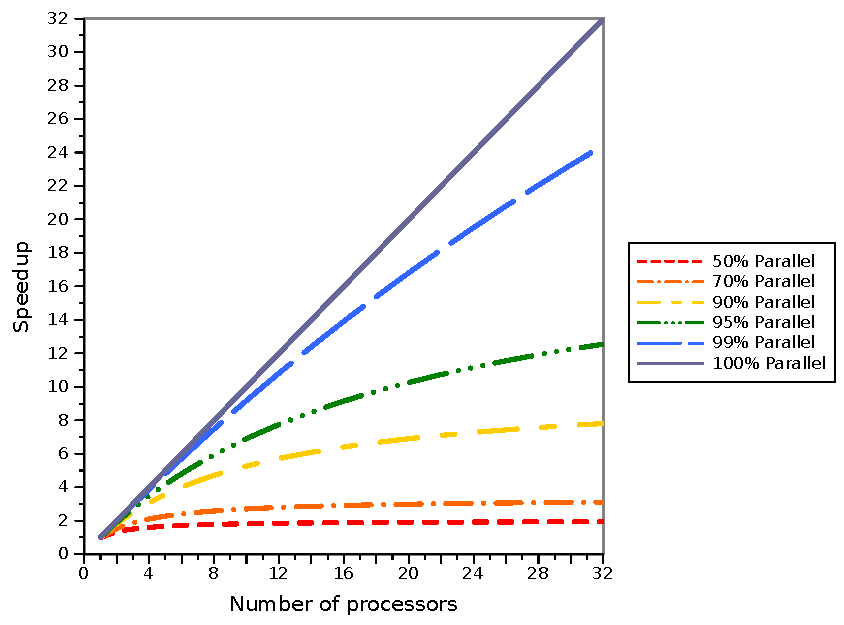
\includegraphics[width=0.5\textwidth]{L02/parallel-scaling}
\end{center}


Amdahl's Law tells you how many cores you can hope to leverage in an
execution given a fixed problem size, if you can estimate $P$.

\paragraph{Consequences of Amdahl's Law.}
For over 30 years, most performance gains did indeed come from
increasing single-processor performance. The main reason that we're
here today is that, as we saw in the video,
single-processor performance gains have hit the wall.

By the way, note that we didn't talk about the cost of synchronization
between threads here. That can drag the performance down even more.

\paragraph{Amdahl's Assumptions.}
Despite Amdahl's pessimism, we still all have multicore computers today.
Why is that? Amdahl's Law assumes that:
\begin{itemize}
    \item problem size is fixed (read on);
    \item the program, or the underlying implementation, behaves the same on 1 processor as on $N$ processors; and
    \item that we can accurately measure runtimes---i.e. that overheads don't matter.
\end{itemize}


\end{document}
